% based on a template made by the university of cologne
% http://www.mi.uni-koeln.de/wp-MIEDV/wp-content/uploads/2016/07/LaTeX-Vorlage.zip - 2023-11-02
\documentclass[12pt,a4paper]{scrartcl}

\addtokomafont{sectioning}{\rmfamily}
\usepackage[ngerman]{babel}% deutsches Sprachpaket wird geladen
\usepackage[T1]{fontenc} % westeuropäische Codierung wird verlangt
\usepackage[utf8]{inputenc}% Umlaute werden erlaubt
\usepackage[usenames]{color} % Erlaubt die Benutzung der namen im Farbpaket und deren Änderung
\usepackage{amsmath} % Erweiterung für den Mathe-Satz
\usepackage{amssymb} % alle Zeichen aus msam und msmb werden dargestellt
\usepackage{graphicx} % Graphiken und Bilder können eingebunden werden
%\usepackage{multirow} % erlaubt in einer Spalte einer Tabelle die Felder in mehreren Zeilen zusammenzufassen
\usepackage{enumerate} % erlaubt Nummerierungen
\usepackage{xurl} % Dient zur Auszeichnung von URLs; setzt die Adresse in Schreibmaschinenschrift.
\usepackage[center]{caption}  % Bildunterschrift wird zentriert
%\usepackage{subfigure} % mehrere Bilder können in einer fugure-Umgebung verwendet werden
%\usepackage{longtable} % Diese Umgebung ist ähnlich definiert wie die tabular-Umgebung, erlaubt jedoch mehrseitige Tabellen.
%\usepackage{paralist} % Modifikation der bereits bestehenden Listenumgebungen
\usepackage{lmodern}% Für die Schrift
\usepackage[hidelinks]{hyperref} % Links und Verweise werden innerhalb von PDF Dokumenten erzeugt
%\usepackage{wrapfig} % Das Paket ermöglicht es von Schrift umflossene Bilder und Tabellen einzufügen.
\usepackage{latexsym} % LaTeX-Symbole werden geladen
\usepackage{tikz} % Erlaubt es mit tikz zu zeichnen
\usepackage{tabularx} % Erlaubt Tabellen
\usepackage{algorithm} % Erlaubt Pseudocode
\usepackage{color} % Farbpaket wird geladen
%\usepackage{stmaryrd} % St Mary Road Symbole werden geladen
\usepackage{physics}
\usepackage{mhchem} % Chemie: \ce & \pu

\numberwithin{equation}{section} % Nummerierungen der Gleichungen, die durch equation erstellt werden, sind gebunden an die section
\newcommand{\HRule}{\rule{\linewidth}{0.7mm}}
\newcommand{\pu}[1]{\ensuremath{\mathrm{#1}}}

% disable commands
\renewcommand{\[}{} % math block start
\renewcommand{\]}{\noindent} % math block end
\newcommand{\tightlist}{} % created in enumerations

\hypersetup{
  pdftitle={B3.4},
  pdfcreator={LaTeX via pandoc}}

\setcounter{secnumdepth}{6}
\setcounter{tocdepth}{6}

\begin{document}
\begin{titlepage}
	\pagestyle{empty}

	\begin{center}

	\textsc{\LARGE Universität zu Köln }\\ [0.4cm]
	\textsc{Mathematisch-Naturwissenschaftliche Fakultät} \\[1.5cm]

	
\includegraphics[width=0.45\textwidth]{../media/uni.jpg}\\[1.5cm]  % Uni-Logo wird geladen

	\textsc{\Large Praktikum~B}\\[2mm]
	\textsc{}\\[10mm]
	\HRule \\[0.4cm]

		{	\Huge \bfseries B3.4}\\[0.4cm]
			{	\huge \bfseries Positronen--Emissions--Tomographie}\\[0.3cm]
	
	\HRule \\[3cm]

 	\begin{center}
		\textsc{\Large Catherine~Tran } \\[3pt]
		\textsc{\Large Carlo~Kleefisch } \\[3pt]
		\textsc{\Large Oliver~Filla } \\[3pt]
	\end{center}
	\end{center}
\end{titlepage}

\newpage
\tableofcontents
\newpage

\hypertarget{einleitung}{%
\section{Einleitung}\label{einleitung}}

Die Positronen--Emissions--Tomographie (PET) ist ein nuklearmedizinisches bildgebendes Verfahren, bei denen radioaktive Materialien als \emph{Tracer} verabreicht werden, die dann im Körper des Patienten gemessen werden. Dadurch können Bilder von z.B. Krebszellen erzeugt werden.

In diesem Versuch wird eine radioaktive Quelle in einer Probe mittels der PET lokalisiert. Weiterhin wird die Ortsauflösung sowie die Winkelabhängigkeit untersucht.

\clearpage
\hypertarget{theoretische-grundlagen}{%
\section{Theoretische Grundlagen}\label{theoretische-grundlagen}}

\hypertarget{pet}{%
\subsection{PET}\label{pet}}

Die Positronen--Emissions--Tomographie ist ein Verfahren, das die Möglichkeit bietet, Veränderungen von Stoffwechselprozessen sowie physiologische Aktivitäten sichtbar zu machen. In der Medizin wird dieses Verfahren hauptsächlich verwendet, um Krebszellen im Körper zu detektieren.

Hierbei injiziert man dem Patienten radioaktive Markerstoffe (\emph{Tracer}). Diese werden unterschiedlich von den Zellen aufgenommen und verarbeitet, abhängig vom lokalen Stoffwechsel. Damit der Körper nicht zu viel radioaktive Strahlungen ausgesetzt wird, muss der Tracer so kurzlebig wie möglich sein und dennoch Positronen abgeben. Deswegen eignen sich z.B. $\ce{^{11}C}$, $\ce{^{13}N}$, $\ce{^{15}O}$,
$\ce{^{18}F}$ besonders. Unterschiedliche Tracer werden für unterschiedliche Körperteile verwendet.

Wenn der Tracer im Gewebe ist, zerfällt er über den $\beta^+$--Zerfall und emittiert dabei Positronen. Innerhalb weniger Mikrometer rekombiniert ein Positron mit einem Elektron und es kommt zur \emph{Paarvernichtung}. Hierbei entstehen zwei Photonen mit jeweils einer Energie von $\pu{511 \,keV}$ ein einem Winkel von $180\,^\circ$ zueinander. $[6]$

Um die Aktivität quantitativ zu bestimmen, werden Signale von den ausgestrahlten Photonen registriert. Wenn zwei davon koinzident sind, hat dieser Prozess mit großer Wahrscheinlichkeit auf der Verbindungslinie\footnote{Englisch: \emph{line of response} (\emph{LOR})} stattgefunden. Aus vielen solcher koinzidenten Signale lässt sich die Aktivität mit einem Computerprogramm zu einem zweidimensionalen und später dreidimensionalen Bild rekonstruieren.

Es kann bei der Messung häufig zu falschen Koinzidenzen kommen. Entweder sind das nur zufällige Signale, die zeitgleich aufgenommen werden, oder das Photon wurde schon auf den Weg zum Detektor gestreut. Diese falsche Koinzidenzen möchte man möglichst gering halten, da sie nicht zur Bildqualität tragen und Nachbearbeitung fordern.

Neben der PET gibt es noch andere bildgebende Verfahren wie Röntgentomographie, Computertomographie (CT), Magnetresonanztomographie (MRT) und Ultraschall. Die Strahlenbelastung ist bei jeweiligem Verfahren unterschiedlich.

Bei Ultraschall werden nur unschädliche Schallwellen verwendet, MRT ist ebenso frei von Strahlenbelastung. Im Vergleich zu Röntgentomographie und CT ist PET weniger schädlich, da die Stoffe sehr schnell zerfallen. Eine Röntgenaufnahme am Brustkorb hat eine Äquivalentdosis von $\pu{0.2 \,mSv}$ und eine CT am Brustkorb hat ca $\pu{8 \,mSv}$ $[8]$.

Laut Bundesamt für Strahlenschutz beträgt der Grenzwert für eine einzelne Person $\pu{1 \,mSv}$ pro Jahr, so lange man nicht beruflich mit Strahlung zu tun hat.

Für die Medizin ist PET ein hervorragendes Werkzeug, besonders in der Onkologie. Das Verfahren kann Veränderung im Stoffwechsel erkennen, eher ein anderes Verfahren es nachweisen kann, so können Krebstumoren früher erkannt und behandelt werden.

\hypertarget{betazerfall}{%
\subsection{\texorpdfstring{$\beta$--Zerfall}{\textbackslash beta--Zerfall}}\label{betazerfall}}

Der $\beta$--Zerfall ist eine der drei Arten radioaktiven Zerfalls. Wie beim $\alpha$--Zerfall wird dabei ein chemisches Element in ein anderes umgewandelt. Im Unterschied zum $\alpha$--Zerfall werden hierbei keine Nukleonen abgesondert, sondern ein Nukleon in ein anderes umgewandelt.

Es wird zwischen drei Arten des $\beta$--Zerfalls unterschieden. Es gibt $\beta^+$--Zerfall und $\beta^-$--Zerfall, weiterhin wird der Elektroneneinfang dazugezählt.

Radioaktiver Zerfall geschieht, wenn der Tochterkern eine höhere Bindungsenergie als der Mutterkern erhält. Hierfür ist insbesondere der Symmetrieterm der Weizsäcker Massenformel $(??)$ interessant. Daran kann man erklären, dass $\beta^-$--Zerfall dann geschehen kann, wenn der Kern mehr Neutronen als Protonen hat.

Umgekehrt kann es zu $\beta^+$--Zerfall kommen, wenn der Kern mehr Protonen als Neutronen hat. Ebenso ist Elektroneneinfang möglich. Welcher dieser Prozesse stattfindet hängt von der Energiedifferenz zwischen Mutterkern und Tochterkern ab: Wenn die Energiedifferenz kleiner als $\Delta E_\mathrm{min}=\pu{1.022 MeV}$ beträgt, dann reicht die Energie nur für Elektroneneinfang. Bei einer Energie von mehr als $\Delta E_\mathrm{min}$ ist auch $\beta^+$--Zerfall möglich. $\Delta E_\mathrm{min}$ entspricht der doppelten Ruheenergie von Elektronen.

Beim $\beta^+$--Zerfall wird ein Proton $p$ in ein Neutron $n$ umgewandelt, dabei entstehen ein Positron $e^+$ sowie ein Elektronenneutrino $\nu_e$. Hierbei wird ein Mutterkern $\ce{^A_Z X}$ in einen Tochterkern $\ce{^A_{Z-1} Y^-}$ umgewandelt. Beim $\beta^-$--Zerfall wird ein Neutron $n$ in ein Proton $p$ umgewandelt, dabei entstehen ein Elektron $e^-$ sowie ein Elektronen--Antineutrino $\bar{\nu}_e$. Hierbei wird ein Mutterkern $\ce{^A_Z X}$ in einen Tochterkern $\ce{^A_{Z+1} Y^+}$ umgewandelt.

Beim Elektroneneinfang (ec) wird ähnlich wie beim $\beta^+$--Zerfall ein Proton $p$ in ein Neutron $n$ umgewandelt. Allerdings wird dazu ein Elektron $e^-$ verwendet, dass aus der $K$--Schale des Atoms eingefangen wurde. Daher wird nur ein Elektronenneutrino $\nu_e$ erzeugt. Hierbei wird ein Mutterkern $\ce{^A_Z X}$ in einen Tochterkern $\ce{^A_{Z-1} Y}$ umgewandelt.

\begin{eqnarray}
    \beta^+:\qquad\,\,\qquad
        \ce{p} &\ce{->}& \quad \ce{n} \quad\, + \ce{e^+} + \ce{\nu_e} \\
        \ce{^A_Z X} &\ce{->}& \ce{^A_{Z-1} Y^-} + \ce{e^+} + \ce{\nu_e} \\
    \beta^-:\qquad\,\,\qquad
        \ce{n} &\ce{->}& \quad \ce{p} \quad\, + \ce{e^-} + \ce{\bar{\nu}_e} \\
        \ce{^A_Z X} &\ce{->}& \ce{^A_{Z+1} Y^+} + \ce{e^-} + \ce{\bar{\nu}_e} \\
    \text{ec}:\qquad
        \ce{p + e^+} &\ce{->}& \quad \ce{n} \ \ \, + \ce{\nu_e} \\
        \ce{^A_Z X} &\ce{->}& \ce{^A_{Z-1} Y} + \ce{\nu_e}
\end{eqnarray}

\noindent
In diesem Versuch wird als Quelle $\ce{^{22}Na}$ verwendet, da eine Halbwertzeit von etwa 2.6 Jahren hat $[2]$. Dieses zerfällt über den $\beta^+$--Zerfall in einen angeregten Zustand des stabilen Nuklides $\ce{^{22}Ne}$, welches unter Aussenden eines $\gamma$--Quants mit $E_\gamma = \pu{1275 keV}$ in den Grundzustand zerfällt, siehe Abbildung \ref{abb:Skizze 22Na}. Beide Zerfälle geschehen koinzident.

\begin{figure}
	\centering
	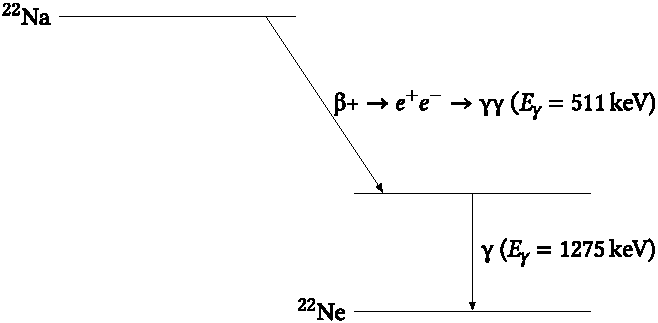
\includegraphics[width=0.7\textwidth]{../media/B3.4/Zerfall_22_Na.pdf}
	\caption{Skizze des Zerfalls von $\ce{^{22}Na}$ zu $\ce{^{22}Ne}$ $[1]$}
	\label{abb:Skizze 22Na}
\end{figure}

\hypertarget{paarvernichtung}{%
\subsection{Paarvernichtung}\label{paarvernichtung}}

Der Begriff der Paarvernichtung beschreibt die Zerstrahlung von einem Teilchen und seinem Antiteilchen, bei der die Teilchen in $\gamma$--Strahlung umgewandelt werden. Die Energie der Strahlung ist die Summe der kinetischen Energie dieser Teilchen sowie ihrer Ruhemassen. Die Paarerzeugung ist der dazu inverse Effekt. $[5]$

Bei der Vernichtung eines Positrons $e^+$ mit einem Elektron $e^-$ entstehen normalerweise zwei $\gamma$--Quanten in einem Winkel $\theta$. Dieser hängt von der transversalen Impulskomponente $p_T$ ab. Weiterhin sind die Ruhemasse $m_e$ der Teilchen und die Lichtgeschwindigkeit $c$ relevant. $[6]$

\begin{eqnarray}
    \tan(\theta) &=& \frac{p_T}{m_ec}
\end{eqnarray}

\noindent
Sind die beiden Teilchen in Ruhe zueinander, so ist der Winkel der $\gamma$--Quanten $\pu{180^\circ}$. Dies liegt an der Impulserhaltung. Ist der Gesamtimpuls vor der Vernichtung $0$, so muss der Gesamtimpuls der beiden $\gamma$--Quanten ebenfalls $0$ sein.

Haben sie einen relativen Impuls, so wird der Winkel kleiner. Sind die Teilchen jedoch zu schnell, dann ist der Wirkungsquerschnitt sehr klein und es ist sehr unwahrscheinlich, dass Paarvernichtung stattfindet.

\hypertarget{gammastrahlung}{%
\subsection{\texorpdfstring{$\gamma$--Strahlung}{\textbackslash gamma--Strahlung}}\label{gammastrahlung}}

Gammastrahlung ist im engeren Sinne eine besonders durchdringende elektromagnetische Strahlung, die bei radioaktivem Zerfall auftritt. Sie wirkt durch drei Prozesse auf Materie. Bei einer Energie von bis zu $E_\gamma = \pu{100 keV}$ überwiegt der Photoeffekt, weiterhin gibt es den Comptoneffekt und Paarbildung.

\hypertarget{photoeffekt}{%
\subsubsection{Photoeffekt}\label{photoeffekt}}

Beim Photoeffekt überträgt ein Photon seine gesamte Energie auf ein Hüllenelektron, welches daraufhin das Atom verlässt. Er wirkt vor allem bei elektromagnetischer Strahlung mit einer Energie von bis zu $E_\gamma = \pu{100 keV}$.

Die kinetische Energie $E_\mathrm{kin}$ des Elektrons hängt von der Energie des Photons $h\nu$ sowie der Austrittsarbeit $W_A$, ab. Letztere ist notwendig, um das Elektron aus dem Atom zu lösen.

\begin{eqnarray}
    E_\mathrm{kin} &=& h\nu - W_A
\end{eqnarray}

\noindent
Der Wirkungsquerschnitt $\sigma_\mathrm{ph}$ wird durch die Ordnungszahl $Z$, die reduzierte Photonenenergie $\epsilon$ $\eqref{redEnergie}$, die Sommerfeld'sche Feinstrukturkonstante $\alpha$ und den Thomson--\allowbreak Wirkungs-querschnitt $\sigma_\mathrm{Th}^e$ bestimmt. $[7]$

\begin{eqnarray}
    \sigma_\mathrm{ph}
        &=& \sqrt{\frac{32}{\epsilon^7}}\alpha^4 Z^5
            \sigma_\mathrm{Th}^e \pu{\frac{cm}{Atom}} \\
    \sigma_\mathrm{ph}
        &\propto& \frac{Z^5}{E_\gamma^{\frac{7}{2}}} \\
    \epsilon &=& \frac{E_\gamma}{m_ec^2} \label{redEnergie} \\
    \sigma_\mathrm{Th}^e &=& \frac{8}{3} \pi r_e^2
\end{eqnarray}

\noindent
Hierbei sind weiterhin die Elektronenmasse $m_e$ und der Radius $r_e$ eines Elektrons relevant.

Da die $\gamma$--Quanten in diesem Versuch im oberen Bereich dieses Energieintervalls liegen, wird der Photoeffekt in diesem Fall zur Ionisation der Atome führen.

\hypertarget{comptoneffekt}{%
\subsubsection{Comptoneffekt}\label{comptoneffekt}}

Der Comptoneffekt tritt vor allem bei $\gamma$--Strahlung mit mittleren Energien von ca. $\pu{100 keV}$ bis $\pu{1 MeV}$ auf. Dabei stößt ein Photon mit einem (quasi--freien) Elektron, wodurch es einen Impuls auf das Elektron überträgt und gestreut wird.

Die Änderung der Wellenlänge $\lambda$ des Photons hängt vom Streuwinkel $\theta$ ab. Der Wirkungsquerschnitt $\sigma_\mathrm{Co}$ ist von der Ordnungszahl $Z$ des Absorbers und der Energie $E_\gamma$ der Strahlung abhängig. $[7]$

\begin{eqnarray}
    \Delta \lambda &=& \frac{h}{m_e c} (1 - \cos(\theta)) \\
    \sigma_\mathrm{Co} &\propto & \frac{Z}{E_\gamma}
\end{eqnarray}

\noindent
Comptoneffekt und Photoeffekt unterscheiden sich in zwei Eigenschaften essenziell. Zum Einen wirkt der Photoeffekt nur auf gebundene, der Comptoneffekt dagegen auf quasifreie Elektronen. Zum Anderen wird beim Photoeffekt die gesamte Energie des Photons aufgebraucht, dagegen wird das Photon beim Comptoneffekt unter Energieverlust gestreut.

\hypertarget{paarbildung}{%
\subsubsection{Paarbildung}\label{paarbildung}}

Bei der Paarbildung entsteht aus einem Photon mit einer hohen Energie ein Teilchen--Antiteilchen--Paar, dieser Effekt dominiert bei Energien von etwa $\pu{5 MeV}$. Die Umkehrung dieses Effektes nennt man Paarvernichtung.

Im Coulombfeld eines Atomkernes kann ein Photon zu einem Positron $e^+$ und einem Elektron $e^-$ zerstrahlen, wenn die Energie des Photons mindestens $\pu{1.022 MeV}$ beträgt. Diese Energie entspricht der Gesamtmasse beider Teilchen.

Der Wirkungsquerschnitt $\sigma_\mathrm{Paar}$ kann wie folgt beschrieben werden. Wie bei dem Photoeffekt sind dabei die Feinstrukturkonstante $\alpha$ und der Elektronenradius $r_e$ relevant, ebenso die reduzierte Energie $\epsilon$ $\eqref{redEnergie}$.

\begin{eqnarray}
    \sigma_\mathrm{Paar}
        &=& 4\alpha r_e^2 Z^2
            \left(\frac{7}{9} \ln(2\epsilon) - \frac{109}{54} \right) \\
    \sigma_\mathrm{Paar}
        &\propto& Z^2 \ln(E_\gamma)
\end{eqnarray}

\hypertarget{impulshuxf6henspektrum}{%
\subsubsection{Impulshöhenspektrum}\label{impulshuxf6henspektrum}}

Die Zahl der in einem~Detektor~nachgewiesenen Ereignisse als Funktion ihrer Impulshöhe wird durch ein Impulshöhenspektrum dargestellt. $[9]$ In Abbildung \ref{abb:Impulshoehenspektrum} ist ein solches für monoenergetische Gamma--Übergänge in $\ce{^{24}Mg}$ dargestellt.

\begin{figure}
	\centering
	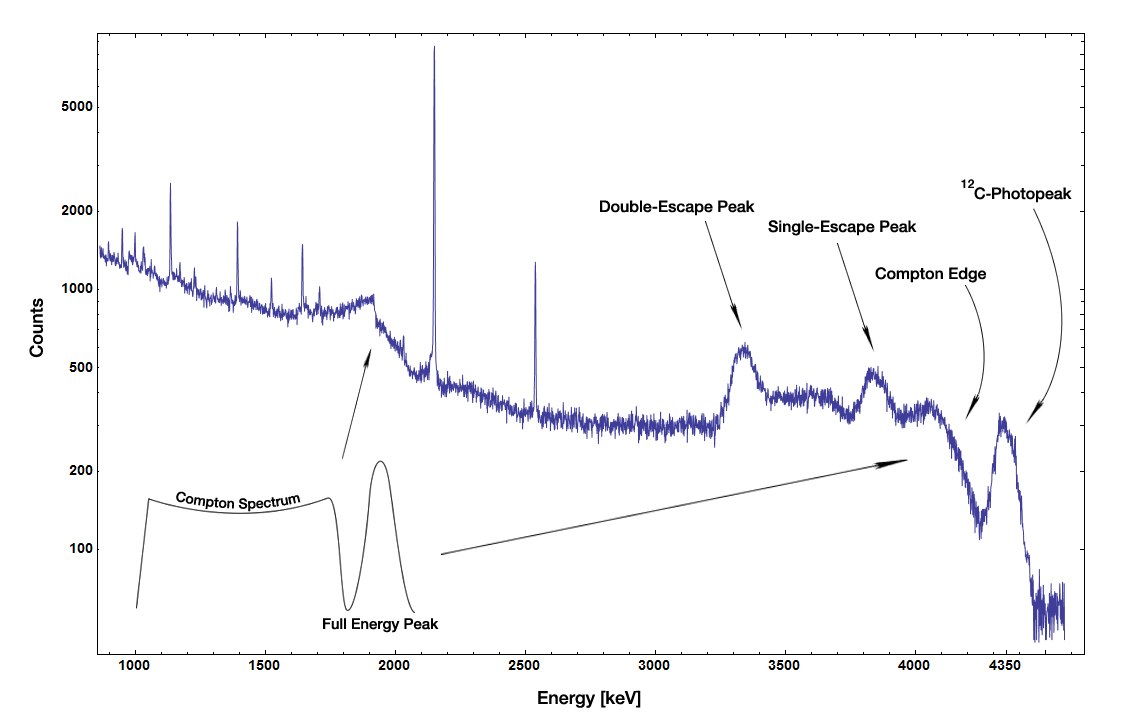
\includegraphics[width=0.9\textwidth]{../media/B3.4/Am_Be_SourceSpectrum.jpg}
	\caption{Impulshöhenspektrum $[7]$}
	\label{abb:Impulshoehenspektrum}
\end{figure}

\paragraph*{Photopeak}

Ein Photopeak (\emph{Full--Energy--Peak}) entsteht, wenn die gesamte Energie eines Photons in einem Detektor gemessen wird. Dies kann beispielsweise durch den bereits genannten Photoeffekt oder durch die Anregung von Atomen entstehen.

\paragraph*{Compton--Kante}

Werden viele Photonen mit der gleichen Energie durch den Comptoneffekt gestreut, so ergibt sich ein charakteristisches Energiespektrum der gestreuten Elektronen, siehe Abbildung \ref{abb:Compton-Kante}. Die hierbei auf die Elektronen übertragene Energie ist eine kontinuierliche Funktion des Streuwinkels~$\phi$, hat jedoch eine scharfe obere Schranke.

\begin{figure}
	\centering
	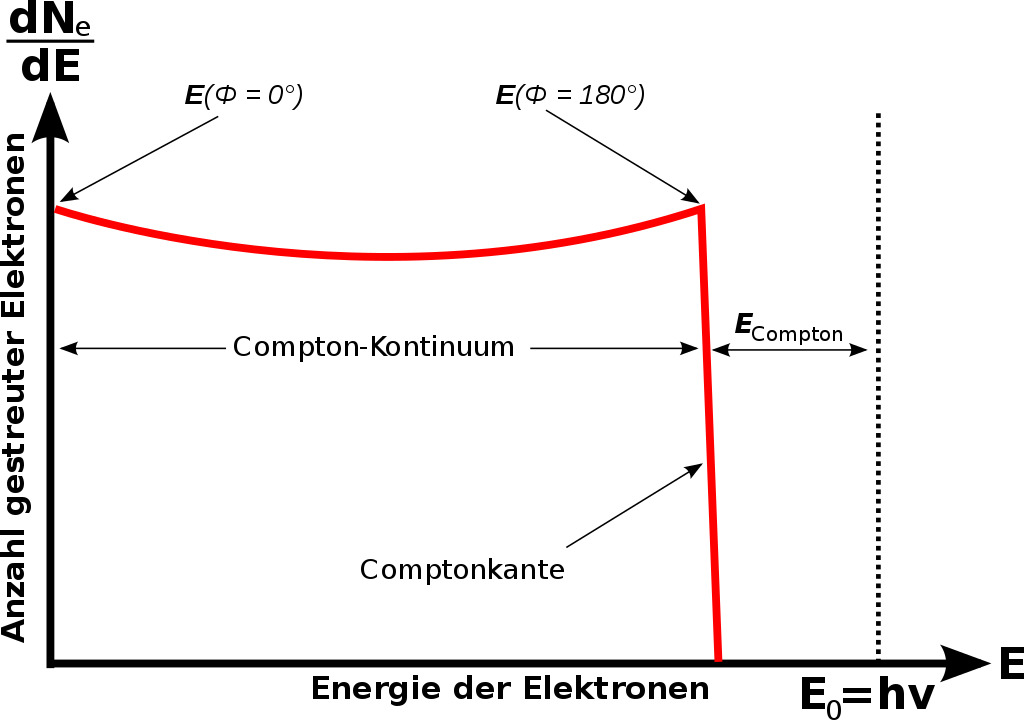
\includegraphics[width=0.7\textwidth]{../media/B3.4/Comptonspektrum.jpg}
	\caption{Compton--Kontinuum und Compton--Kante $[10]$}
	\label{abb:Compton-Kante}
\end{figure}

Das Compton--Kontinuum $E_e'(\phi)$ beschreibt den Energie des Elektrons nach dem Stoß $\eqref{Compton--Kontinuum}$, die obere Schranke derselben ist die \emph{Compton--Kante} $E_e(180^\circ)$ $\eqref{Compton--Kante}$. Die Energie des Photons nach der Streuung $E_{\gamma}^\prime(\phi)$ wird dagegen durch die Klein--Nishina--Formel $\eqref{Klein--Nishina}$ beschrieben.

\begin{eqnarray}
    E_e^\prime(\phi)
        &=& E_{\gamma} - E_{\gamma}'(\phi) \\
        &=& E_{\gamma}
            \left(
                1-
                \frac{1}{1+\frac{E_{\gamma}}{m_\mathrm ec^2}
                    (1-\cos(\phi))}
            \right) \label{Compton--Kontinuum} \\
    E_e^\prime(180^\circ) &=& \frac{E_\gamma}{1+\frac{m_ec^2}{2E_\gamma}}
        \label{Compton--Kante} \\
    E_{\gamma}^\prime(\phi)
        &=& \frac{E_{\gamma}}{1+\frac{E_{\gamma}}{m_\mathrm ec^2}
            (1-\cos\phi)} \label{Klein--Nishina}
\end{eqnarray}

\paragraph*{Rückstreupeak}

Ein Compton--Rückstreuungspeak (\emph{Backscatter Peak})~tritt bei der Energie $E_\mathrm{Rück}$ auf, wenn die $\gamma$--Strahlen in das Material um den Detektor herum gestreut wurden und erst danach in den
den Detektor treffen. $[7]$

\begin{eqnarray}
    E_\mathrm{Rück} &=& E_\gamma - E_e^\prime(180^\circ)
\end{eqnarray}

\paragraph*{Escapelinien}

Escapelinien oder Escape--Peaks sind unechte Spektrallinien, die bei der Röntgen- und Gammaspektroskopie auftreten und z.B. die Anwesenheit nicht vorhandener Radionuklide in der gemessenen Probe vortäuschen können. $[16]$

Gammastrahlung mit einer Energie von $E_\gamma\ge\pu{1022MeV}$ kann zur Paarbildung führen. Dabei entstehende Positronen zerstrahlen wiederum mit anderen Elektronen. Dies kann auch in einem Detektor geschehen. Es ist dabei nicht garantiert, dass die dabei entstehenden $\gamma$-Quanten detektiert werden. $[7]$

Wenn nur ein Photon detektiert wird, verursacht dies einen \emph{Single--Escape--Peak} bei einer Energie von
$E_\gamma - \pu{511 keV}$. Wird keines der Photonen detektiert, gibt es einen \emph{Double--Escape--Peak} bei der Energie $E_\gamma - \pu{1022 keV}$.

\hypertarget{elektronik}{%
\subsection{Elektronik}\label{elektronik}}

In diesem Versuch werden verschiedene elektronische Bauteile verwendet, die im Folgenden näher erläutert werden. Ein Schaltskizze des Versuchs lässt sich in Abbildung \ref{abb:Schaltplan} finden.

\begin{figure}
	\centering
	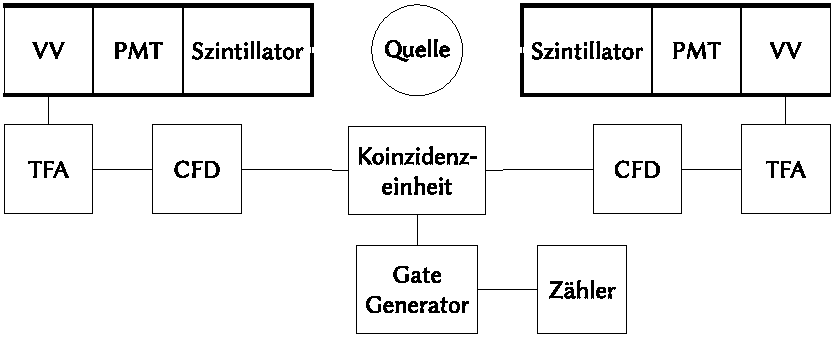
\includegraphics[width=0.85\textwidth]{../media/B3.4/Schaltplan.pdf}
	\caption{Schaltskizze des Versuchs $[1]$, bestehend aus
		Photomultiplier (PMT), Vorverstärker (VV),
		Hauptverstärker (TFA) und Diskriminator (CFD)}
	\label{abb:Schaltplan}
\end{figure}

Als Detektor für die koinzidenten Signale werden anorganische Szintillationszähler sowie Photomultiplier zur Elektronenvervielfachung verwendet.

In diesem Versuch wird $\ce{NaI}$ als anorganischer Szintillator verwendet, hierbei beträgt die Ausbeute je Photon $\pu{4\cdot 10^{4} MeV^{-1}}$.

\hypertarget{verstuxe4rker}{%
\subsubsection{Verstärker}\label{verstuxe4rker}}

Ein Verstärker wird dazu verwendet ein eintreffendes elektronisches Signal zu verstärken. Dabei wird zwischen Vor- und Hauptverstärker unterschieden.

Ein Vorverstärker wird direkt an die Detektoren angeschlossen, oder die Detektoren haben, wie in diesem Versuch, bereits einen Vorverstärker integriert. Dieser dient dazu, das von den Detektoren stammende Signal
zu verstärken, sodass die Verluste in den Kabeln, die den Detektor mit den anderen Bauteilen verbinden, minimiert werden.

Der in diesem Versuch verwendete Hauptverstärker, ein \emph{Timing Filter Amplifier} (TFA), dient dazu, dem Signal eine möglichst kurze Anstiegsflanke zu verleihen. Er empfängt das Signal aus den Vorverstärkern, verstärkt es und leitet es weiter zu den Diskriminatoren.

Alternativ kann man einen \emph{Spectroscopy Amplifier} (SA) als Hauptverstärker nutzen, der das Signal möglichst verzerrungsfrei verstärkt. Dies ist für Messungen interessant, in denen die Energieauflösung wichtiger als die Zeitauflösung ist.

\hypertarget{diskriminator}{%
\subsubsection{Diskriminator}\label{diskriminator}}

Ein Diskriminator ist ein Bauteil, das ein logisches Signal\footnote{Ein logisches Signal ist ein Kastensignal, das nur zwei verschiedene Werte annimmt.} einer gewissen Breite ausgibt, falls die Amplitude des eintreffenden Signals eine einstellbare Schwelle überschreitet.

Da in diesem Versuch die Messung von zwei koinzidenten $\gamma$--Quanten relevant ist, ist es wichtig, dass die Diskriminatoren die logischen Signale zweier zeitgleich eintreffenden Signale auch zeitgleich ausgeben. Dabei gibt es jedoch zwei Probleme, den \emph{Walk} und den \emph{Jitter}.

\paragraph*{Walk}
Treffen zwei Signale zeitgleich in zwei Detektoren ein, haben aber unterschiedliche maximale Amplituden, erreichen diese beiden Signale die Amplituden--Schwelle der Diskriminatoren zu unterschiedlichen Zeitpunkten. Dies ist in Abbildung \ref{abb:Walk-Effekt} dargestellt.

Die von den Diskriminatoren ausgesendeten logischen Signale sind dadurch zeitverschoben, obwohl die eintreffenden Signale koinzident waren. Diese Verschiebung der logischen Signale wird \emph{Walk} genannt.

\begin{figure}
	\centering
	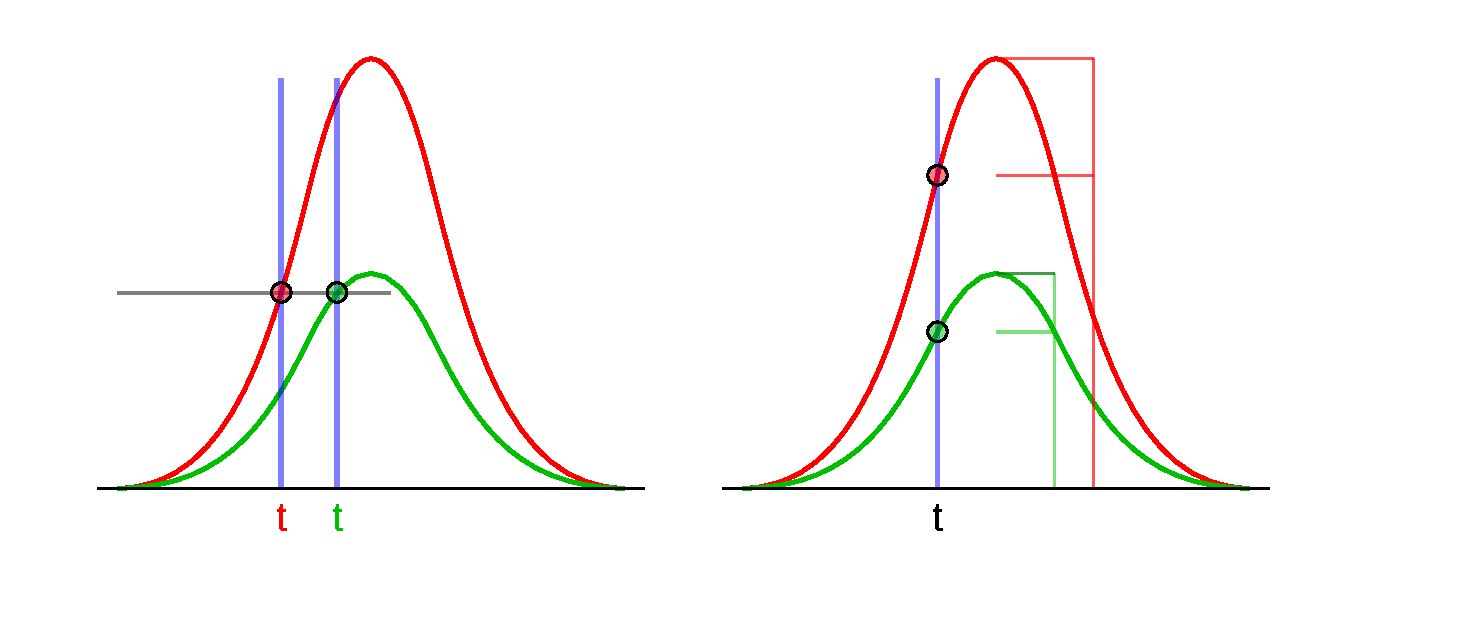
\includegraphics[width=0.7\textwidth]{../media/B3.4/Constant_fraction_1.pdf}
	\caption{Links: Walk--Effekt, Rechts: Kein Walk--Effekt}
	\label{abb:Walk-Effekt}
\end{figure}

\hypertarget{jitter}{%
\paragraph*{Jitter}\label{jitter}}

Aufgrund von statistischen Fluktuationen und Untergrundrauschen kann es passieren, dass zwei eigentlich gleiche Signale einen unterschiedlichen Zeitverlauf aufweisen. Daraufhin kann sich wie schon beim Walk der Zeitpunkt unterscheiden, bei dem die Signale die Amplituden--Schwelle der Diskriminatoren erreichen, wodurch die ausgesendeten logischen Signale wieder zeitversetzt sind. Dieses Phänomen wird als \emph{Jitter} bezeichnet.

\hypertarget{cfd}{%
\subsubsection{Constant--Fraction--Diskriminator}\label{cfd}}

Um den Problemen durch Walk und Jitter entgegenzuwirken, wird in diesem Versuch ein \emph{Constant--Fraction--Diskriminator} (CFD) verwendet. Ein CFD teilt ein eintreffendes Signal in zwei Teilsignale. Das erste Teilsignal wird um eine gewisse Zeit $T$ verzögert. Das zweite Teilsignal wird invertiert und um einen Faktor $k\in(0, 1)$ gestaucht. Daraufhin werden beide Teilsignale wieder addiert. Der CFD sendet das logische Signal dann erst aus, wenn das wie oben beschrieben veränderte Signal seinen Nulldurchgang erreicht. Es ist in Abbildung \ref{abb:CFD} dargestellt.

\begin{figure}
	\centering
	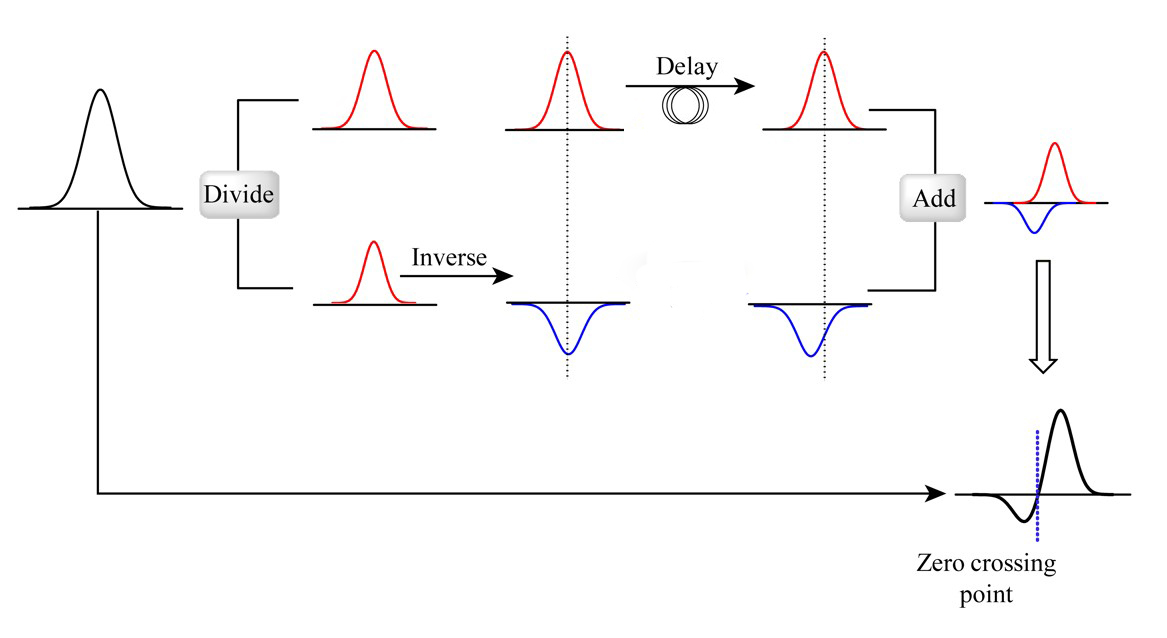
\includegraphics[width=0.7\textwidth]{../media/B3.4/CFD.jpg}
	\caption{Funktionsprinzips eines Constant--Fraction--Diskriminators $[15]$}
	\label{abb:CFD}
\end{figure}

\hypertarget{koinzidenzeinheit}{%
\subsubsection{Koinzidenzeinheit}\label{koinzidenzeinheit}}

Die logischen Signale aus den beiden Diskriminatoren werden dann gemeinsam zur Koinzidenzeinheit weitergeleitet. Diese überprüft, ob sich die beiden Signale überlappen. Falls dies der Fall ist, sendet sie ein logisches Signal an einen \emph{Gate Generator}, der das Signal in ein genormtes logisches Signal umformt. Dieses wiederum wird an den Zähler weitergegeben.

\hypertarget{szintillatoren}{%
\subsubsection{Szintillatoren}\label{szintillatoren}}
Wenn Photonen auf ein Szintillationsmaterial treffen, wechselwirken sie und regen die Elektronen an. Nach einer Zeit fallen diese wieder in den Grundzustand ab und senden dabei Licht im sichtbaren Bereich aus. Die Zeit dieses Ablaufs beträgt abhängig vom verwendeten Material zwischen $\pu{100 ps}$ und $\pu{1\mu s}$.

Wenn Photonen auf den Szintillationskristall treffen, wird die Energie des Photons auf Elektronen im Valenzband übertragen und die Elektronen werden ins Leitungsband angehoben. Fallen sie wieder zurück ins Valenzband, wird erneut ein Photon mit derselben Energie emittiert. Mit sehr hoher Wahrscheinlichkeit wird dieses Photons wieder direkt von einem anderen Elektron im Valenzband absorbiert, dies kann unendlich oft passieren.

Um diesem endlosen Effekt entgegenzuwirken dotiert man den Kristall so, dass die Bandlücke lokal durch Energiezustände von diesen Atomen verkleinert wird. Die Elektronen können dann in verschiedene Zuständen zwischen Valenz- und Leitungsband fallen und emittieren dabei Photonen im sichtbaren Bereich. Diese Photonen haben aber nicht mehr die Größe der vorherrschenden Bandlücke und werden daher auch nicht wieder absorbiert.

Diese Photonen treffen dann auf die Kathode des Photomultipliers, welcher im nächsten Kapitel erläutert wird.

Häufig sind Szintillatoren anorganische Isolatoren oder Halbleiter mit einer großen Bandlücke. Der Vorteil von anorganischen Szintillatoren aus Kristall oder Glas ist die hohe Lichtausbeute, welche sehr wichtig für die Energiemessgenauigkeit ist. Nachteilig dagegen ist die langsame Lichtemission im Bereich von einigen $\pu{100 ns}$, die Energieauflösung sowie die Feuchtigkeitsempfindlichkeit von manchen Kristallen.

Ein Photon aus einem Paarvernichtungsprozess mit einer Energie von $\pu{511keV}$ kann zehntausende Elektronen anregen, da diese mit Energien im $\pu{eV}$--Bereich gebunden sind. Beim Wasserstoff ist das Elektron mit $\pu{13.6eV}$ gebunden, hier könnten theoretisch bis zu $35.6\cdot 10^3$ Photonen angeregt werden.

Weiterhin gibt es organische Szintillatoren, die haupsächlich aus langen Kohlenstoffketten bestehen. Das Licht wird durch zwei Hauptprozesse erzeugt, die Floureszenz und die Phosphoreszenz.

Floureszenz ist ein Prozess, bei dem ein absorbiertes Photon nach Anregung sofort wieder abgestrahlt wird, dies erfolgt durch einen erlaubten Übergang zwischen zwei Zuständen.

Der Prozess der Phosphoreszenz läuft dagegen langsamer ab, weil ein verbotener Übergang zwischen einem angeregten Zustand und dem Grundzustand durch eine Multipol--Auswahlregel stattfinden muss. Im Allgemeinen kommt das Lichtsignal in einem organischen Szintillator früher als im anorganischen, im Idealfall kommt es schon nach $\pu{100 ps}$. Trotz diesem Vorteil haben sie nur eine geringe Lichtausbeute. $[13]$

\hypertarget{photomultiplier}{%
\subsubsection{Photomultiplier}\label{photomultiplier}}

Um aus dem Szintillationslicht ein Messsignal zu erhalten, schließt man dem Szintillator einen Photomultiplier an. Dieser besteht aus einer Photokathode und einem Sekundärelektronenvervielfacher. Dabei muss das Emissionspektrum des Detektors optimal auf die spektrale Empfindlichkeit der Photokathode abgestimmt sein.

Die Kathode besteht entweder aus Alkali--Metallen oder Erdalkali--Metallen, die über eine geringe Elektronenaustrittarbeit verfügen.

Der zweite Bauteil heißt Sekundärelektronenvervielfacher\footnote{\emph{photomultiplier tube} (PMT)} (SEV). Dieser besitzt eine Folge von Elektroden, genannt Dynoden, die bis zu $10^7$ Sekundärelektronen pro Primärelektron erzeugen können. Zwischen den einzelnen Dynoden wird ein elektrisches Potenzial angelegt, sodass die Elektronen bis zur Anode hin beschleunigt werden. Üblicherweise haben SEVs ca. $10$ Dynoden, mit jedem Auftreffen auf eine davon werden Sekundärelektronen heraus geschlagen und vervielfacht.

Die ganze Elektronik befindet sich in einem vakuumdichten Glaskolben, der zusätzlich mit einem $\mu$--Metall--Zylinder gegen magnetische Streufelder abgeschirmt ist $[13]$. Abbildung \ref{abb:Photomultiplier} zeigt den Aufbau von einem typischen Photomultiplier.

Das messbare Signal an der Anode ist dann durch richtige Kalibrierung proportional zu der im Szintillationskristall deponierten Energie des Photons aus dem $e^+ e^-$--Annihilationprozess.

\begin{figure}
	\centering
	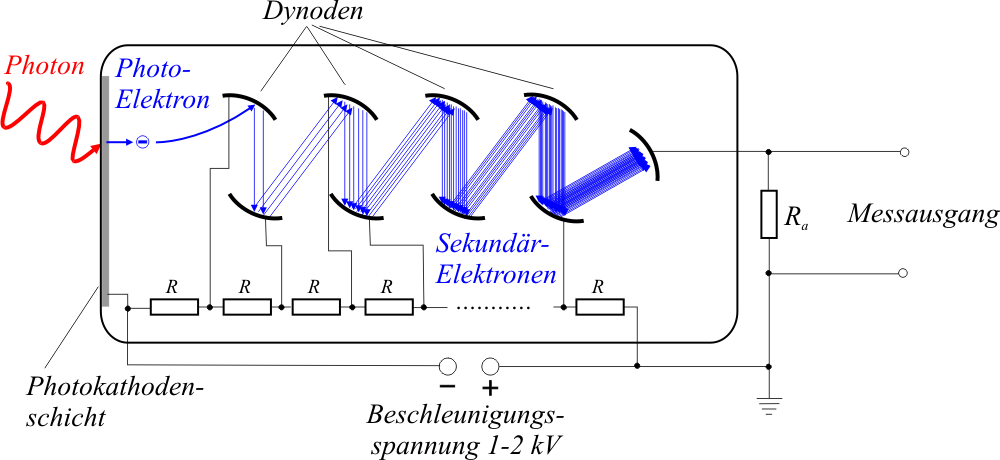
\includegraphics{../media/B3.4/Photomultiplier_schema_de.png}
	\caption{Photomultiplier (schematisch) $[12]$}
	\label{abb:Photomultiplier}
\end{figure}

\hypertarget{weizsuxe4cker-massenformel}{%
\subsection{Weizsäcker Massenformel}\label{weizsuxe4cker-massenformel}}
Die \emph{Weizsäcker Formel} gibt die Bindungsenergie eines Atomkerns an. Sie basiert einerseits auf empirischen Daten, andererseits auf dem Tröpfchenmodell. Aus ihr wird die Weizsäcker Massenformel ermittelt.

Das Tröpfchenmodell beschreibt einen Atomkern als einen inkompressiblen, kugelförmigen Fluidtropfen, der zur Energieminimierung den Kernradius $R$ aufweist. Dabei ist die Dichte überall konstant.

Die Bindungsenergie $E_B$ wird aus fünf verschiedenen Termen ermittelt, auf die im Folgenden eingegangen wird. Diese Terme werden durch die empirisch ermittelten Faktoren $a_i$ sowie die Nukleonenzahl bzw. Massenzahl $A$, Protonenzahl $Z$ und Neutronenzahl $N$ beschrieben. Hierbei handelt es sich um den Volumenterm $E_V$ $\eqref{Volumenterm}$, den Oberflächenterm $E_O$ $\eqref{Oberflächenterm}$, den Coulombterm $E_C$ $\eqref{Coulombterm}$, den Symmetrieterm $E_S$ $\eqref{Symmetrieterm}$ und den Paarungsterm $E_P$ $\eqref{Paarungsterm}$.

\begin{eqnarray}
	E_B &=& E_V + E_O + E_C + E_S + E_P
\end{eqnarray}

\noindent
Die Bindungsenergie $E_B$ verringert die Masse des Atomkernes. Daher kann die Kernmasse $m$ durch die Protonenmasse $m_P$, die Neutronenmasse $n_N$ sowie $E_B$ beschrieben werden, wobei die Lichtgeschwindigkeit $c$ die Energie in Masse konvertiert. Dies ergibt die \emph{Weizsäcker Massenformel}.

\begin{eqnarray}
	m &=& N\cdot m_N + P\cdot m_P - \frac{E_B}{c^2}
\end{eqnarray}

\noindent
In der Darstellung der einzelnen Terme ist weiterhin relevant, dass der Kernradius $R$ kann durch den Radius $r$ eines Nukleons und die Nukleonenzahl $A$ beschrieben werden kann.

\begin{eqnarray}
	R &=& r \cdot \sqrt[3]{A}
\end{eqnarray}

\hypertarget{volumenterm}{%
	\paragraph{Volumenterm}\label{volumenterm}}

Der Volumenterm $E_V$ beschreibt die Anziehung der Nukleonen durch die starke Wechselwirkung.

Diese hat eine Reichweite von $2.5\mathrm{\,fm}$, weswegen sie nur auf die nächsten Nachbarn eines Nukleons wirkt. Da die Dichte im Kern nach dem Tröpfchenmodell konstant ist, ist die gesamte Bindungsenergie durch die starke Wechselwirkung proportional zum Kernvolumen. Dieses wiederum ist proportional zu $R^3\propto A$.

\begin{eqnarray}
	E_V &=& + a_V\cdot A \label{Volumenterm} \\
	a_V &=& 15.85\mathrm{\,MeV}
\end{eqnarray}

\hypertarget{oberfluxe4chenterm}{%
	\paragraph{Oberflächenterm}\label{oberfluxe4chenterm}}

Da die Atome an der Oberfläche des Atomkerns weniger Nachbarn haben als die Nukleonen im Kern, wird sind die ersteren schwächer gebunden. Daher beschreibt der Oberflächenterm $E_O$ eine Korrektur des Volumenterms. Diese ist proportional zur Oberfläche einer Kugel mit dem Kernradius $R$, also proportional zu $\sqrt[3]{A^2}$.

\begin{eqnarray}
	E_O &=& - a_O\cdot \sqrt[3]{A^2} \label{Oberflächenterm} \\
	a_O &=& 18.34\mathrm{\,MeV}
\end{eqnarray}

\hypertarget{coulombterm}{%
	\paragraph{Coulombterm}\label{coulombterm}}

Der Coulombterm $E_C$ beschreibt die elektrostatische Abstoßung der Protonen voneinander, die die Bindungsenergie senkt. Jedes der $Z$ Protonen wird von den anderen $(Z-1)$ Protonen abgestoßen. Die Coulombwechselwirkung ist proportional zu $R^{-1}\propto\left(\sqrt[3]{A}\right)^{-1}$.

\begin{eqnarray}
	E_C &=& - a_C\cdot \frac{Z(Z-1)}{\sqrt[3]{A}} \label{Coulombterm} \\
	a_C &=& 0.71\mathrm{\,MeV}
\end{eqnarray}

\noindent
Für große Kerne mit $Z\approx(Z-1)$ kann der Term $Z(Z-1)\approx Z^2$ vereinfacht werden.

\hypertarget{symmetrieterm}{%
	\paragraph{Symmetrieterm}\label{symmetrieterm}}

Der Symmetrieterm $E_S$ beschreibt die Verringerung der Bindungsenergie durch ein Ungleichgewicht von Protonen und Neutronen.

Die Ursache kann quantenmechanisch erklärt werden. Protonen und Neutronen werden als Fermigas in einem Potentialtopf betrachtet. Beide Gase teilen sich denselben Potentialtopf und füllen Einteilchenniveaus bis zu ihrer jeweiligen Fermienergie auf. Sind genau gleich viele beider Teilchensorten vorhanden, so sind alle Zustände bis zur Fermienergie besetzt.

Gibt es jedoch ein Teilchen mehr von einer Sorte, so müssen höhere Energieniveaus besetzt werden. Sei z.B. ein Proton mehr vorhanden, so muss ein Proton ein höheres Energieniveau als alle anderen Nukleonen besetzen. Dies benötigt mehr Energie.

Wandelt man nun in einem symmetrischen Kern ein Nukleon um, so erhöht man die eine Fermienergie und senkt die andere ab. Dieser Prozess kostet Energie, der Betrag der Energie ist die Differenz zwischen den Ferminiveaus. Wenn man die Energiedifferenz in einer Tabelle aufträgt, sieht man, dass der Term erst am Anfang mit $(N-Z)$ wächst und bei Umschichtungen von drei Nukleonen eine besser Beschreibung das Wachstum mit $(N-Z)/2$ ist. Wenn man dann noch betrachtet, dass Abstand der Einteilchenniveaus mit steigendem Volumen sinkt, erhält man mit der Proportionalität zwischen Volumen und Nukleonenzahl $A$ folgende Formel.

\begin{eqnarray}
	E_S &=& - a_S\cdot \frac{(N-Z)^2}{4A} \label{Symmetrieterm} \\
	a_S &=& 2.86\mathrm{\,MeV}
\end{eqnarray}

\hypertarget{paarungsterm}{%
	\paragraph{Paarungsterm}\label{paarungsterm}}

Der Paarungsterm $E_P$ beschreibt das Phänomen, dass gerade Anzahlen von Protonen bzw. Neutronen in einem Kern stabilere Kerne produzieren. Paare von Protonen oder Neutronen sind stärker gebunden als ein ungepaartes Proton oder Neutron.

Deswegen wird zwischen $\mathrm{gerade}$--$\mathrm{gerade}$--Kernen $(\mathrm{gg})$, $\mathrm{gerade}$--$\mathrm{ungerade}$--Kernen $(\mathrm{gu})$ und $\mathrm{ungerade}$--$\mathrm{gerade}$--Kernen $(\mathrm{ug})$ sowie $\mathrm{ungerade}$--$\mathrm{ungerade}$--Kernen $(\mathrm{uu})$ unterschieden. Erstere haben jeweils eine gerade Anzahl von Protonen und Neutronen, während letztere jeweils ungerade Anzahlen haben. $\mathrm{ug}$-- und $\mathrm{gu}$--Kerne haben eine Nukleonensorte in gerader und die andere in ungerader Menge.

Bei einer geraden Anzahl derselben Nukleonensorte heben sich die Spins auf, bei einer ungeraden Anzahl nicht. Auf diese Weise kann das Phänomen mithilfe des Schalenmodells erklärt werden.

Der Paarungsterm wird betragsmäßig kleiner, je größer die Nukleonenzahl $A$ ist. Dies wird durch die folgende Gleichung beschrieben.

\begin{eqnarray}
	E_P &=&
	\begin{cases}
		+ a_P\cdot \frac{1}{\sqrt{A}} & \text{gg} \\
		0 & \text{gu} \\
		0 & \text{ug} \\
		- a_P\cdot \frac{1}{\sqrt{A}} & \text{uu} \\
	\end{cases}
	\label{Paarungsterm} \\
	a_P &=& 11.46\mathrm{\,MeV}
\end{eqnarray}

\noindent
Beide Nukleonensorten liefern betragsmäßig den gleichen Beitrag zu $E_P$. Bei $\mathrm{gg}$-- und $\mathrm{uu}$--Kernen addieren sich diese Werte zu einer nicht--verschwindenden Energie. Bei $\mathrm{gu}$-- und $\mathrm{ug}$--Kernen heben sich die Terme dagegen auf, weswegen der Paarungsterm hier verschwindet.


\clearpage
\hypertarget{durchfuxfchrung}{%
\section{Durchführung}\label{durchfuxfchrung}}

\hypertarget{ortsaufluxf6sung}{%
\subsection{Ortsauflösung}\label{ortsaufluxf6sung}}
Es soll die Ortsauflösung der Koinzidenzmessung bestimmt werden. Dazu wurde die Quelle mittig auf dem Wagen positioniert. Daraufhin wurde der Wagen auf verschiedene Positionen im Bereich von $\pm 50\,\mathrm{mm}$ eingestellt und bei verschiedenen Positionen die Zählraten für jeweils $T_\mathrm{Ort}=60\,\mathrm{s}$ gemessen.

In den Abständen von $\pm 8\,\mathrm{mm}$ wurden minimale Abstände von $\pm 1\,\mathrm{mm}$ zwischen den Positionen verändert, weiter außen wurden größere Abstände gewählt. Die Ungenauigkeit beim Einstellen der Position wird auf $\pu{\pm 2 mm}$ gesetzt.

\hypertarget{petscan}{%
\subsection{PET--Scan}\label{petscan}}


\begin{align*}
    &x_1 = \pu{(-45\pm2) mm} &&
        N(x_1) = 190 \\
    &x_2 = \pu{(-35\pm2) mm} &&
        N(x_2) = 261 \\
    &x_3 = \pu{(-25\pm2) mm} &&
        N(x_3) = 440 \\
    &x_4 = \pu{(-15\pm2) mm} &&
        N(x_4) = 312 \\
    &x_5 = \pu{(-5\pm2) mm} &&
        N(x_5) = 414 \\
    &x_6 = \pu{(5\pm2) mm} &&
        N(x_6) = 639 \\
    &x_7 = \pu{(15\pm2) mm} &&
        N(x_7) = 2025 \\
    &x_8 = \pu{(25\pm2) mm} &&
        N(x_8) = 616 \\
    &x_9 = \pu{(35\pm2) mm} &&
        N(x_9) = 660 \\
    &x_{10} = \pu{(45\pm2) mm} &&
        N(x_{10}) = 2186
\end{align*}

\begin{align*}
    &y_1 = \pu{(-45\pm2) mm} &&
        N(y_1) = 313 \\
    &y_2 = \pu{(-35\pm2) mm} &&
        N(y_2) = 466 \\
    &y_3 = \pu{(-25\pm2) mm} &&
        N(y_3) = 542 \\
    &y_4 = \pu{(-15\pm2) mm} &&
        N(y_4) = 2021 \\
    &y_5 = \pu{(-5\pm2) mm} &&
        N(y_5) = 498 \\
    &y_6 = \pu{(5\pm2) mm} &&
        N(y_6) = 481 \\
    &y_7 = \pu{(15\pm2) mm} &&
        N(y_7) = 431 \\
    &y_8 = \pu{(25\pm2) mm} &&
        N(y_8) = 503 \\
    &y_9 = \pu{(35\pm2) mm} &&
        N(y_9) = 2385 \\
    &y_{10} = \pu{(45\pm2) mm} &&
        N(y_{10}) = 520
\end{align*}

\begin{align*}
    &z_{1} = \pu{(64\pm2) mm} &&
        N(z_{1}) = 203 \\
    &z_{2} = \pu{(57\pm2) mm} &&
        N(z_{2}) = 246 \\
    &z_{3} = \pu{(49\pm2) mm} &&
        N(z_{3}) = 243 \\
    &z_{4} = \pu{(42\pm2) mm} &&
        N(z_{4}) = 271 \\
    &z_{5} = \pu{(35\pm2) mm} &&
        N(z_{5}) = 318 \\
    &z_{6} = \pu{(28\pm2) mm} &&
        N(z_{6}) = 407 \\
    &z_{7} = \pu{(21\pm2) mm} &&
        N(z_{7}) = 644 \\
    &z_{8} = \pu{(14\pm2) mm} &&
        N(z_{8}) = 1907 \\
    &z_{9} = \pu{(7\pm2) mm} &&
        N(z_{9}) = 556 \\
    &z_{10} = \pu{(0\pm2) mm} &&
        N(z_{10}) = 486 \\
    &z_{11} = \pu{(-7\pm2) mm} &&
        N(z_{11}) = 524 \\
    &z_{12} = \pu{(-14\pm2) mm} &&
        N(z_{12}) = 397 \\
    &z_{13} = \pu{(-21\pm2) mm} &&
        N(z_{13}) = 384 \\
    &z_{14} = \pu{(-28\pm2) mm} &&
        N(z_{14}) = 401 \\
    &z_{15} = \pu{(-35\pm2) mm} &&
        N(z_{15}) = 562 \\
    &z_{16} = \pu{(-42\pm2) mm} &&
        N(z_{16}) = 2173 \\
    &z_{17} = \pu{(-49\pm2) mm} &&
        N(z_{17}) = 571 \\
    &z_{18} = \pu{(-57\pm2) mm} &&
        N(z_{18}) = 390 \\
    &z_{19} = \pu{(-64\pm2) mm} &&
        N(z_{19}) = 306 \\
\end{align*}

An den Positionen $(7,8)$ und $(10,4)$ sind ziemlich sicher Proben,
die Probe bei $(3, 2)$ war ebenfalls eine Probe, dies fanden wir an
den Werten allerdings schwer zu erkennen.

\hypertarget{winkelabhuxe4ngigkeit}{%
\subsection{Winkelabhängigkeit}\label{winkelabhuxe4ngigkeit}}

Im Folgenden wird die Winkelabhängigkeit sowohl von dem
$\pu{511keV}$--Peak der Annihilation als auch von dem
$\pu{1275keV}$--Peak aus dem sekundären Zerfall ermittelt. Bei
ersterem wird eine starke Winkelabhängigkeit erwartet, bei letzterem
keine Winkelabhängigkeit.

Der Fehler des Winkels wird auf $\Delta \theta = \pu{0.5^\circ}$
geschätzt.

\hypertarget{pu511kevpeak}{%
\subsubsection{\texorpdfstring{$\pu{511keV}$--Peak}{\textbackslash pu\{511keV\}--Peak}}\label{pu511kevpeak}}

\begin{eqnarray*}
    N(-5.0^\circ) &=& 432 \\
    N(-4.5^\circ) &=& 476 \\
    N(-4.0^\circ) &=& 484 \\
    N(-3.5^\circ) &=& 585 \\
    N(-3.0^\circ) &=& 885 \\
    N(-2.5^\circ) &=& 707 \\
    N(-2.0^\circ) &=& 1007 \\
    N(-1.5^\circ) &=& 1646 \\
    N(-1.0^\circ) &=& 2147 \\
    N(-0.5^\circ) &=& 2559 \\
    N(\pm0.0^\circ) &=& 2462 \\
    N(+0.5^\circ) &=& 1946 \\
    N(+1.0^\circ) &=& 1383 \\
    N(+1.5^\circ) &=& 1075 \\
    N(+2.0^\circ) &=& 637 \\
    N(+2.5^\circ) &=& 533 \\
    N(+3.0^\circ) &=& 444 \\
    N(+3.5^\circ) &=& 494 \\
    N(+4.0^\circ) &=& 503 \\
    N(+4.5^\circ) &=& 471 \\
    N(+5.0^\circ) &=& 456
\end{eqnarray*}

\hypertarget{pu1275kevpeak}{%
\subsubsection{\texorpdfstring{$\pu{1275keV}$--Peak}{\textbackslash pu\{1275keV\}--Peak}}\label{pu1275kevpeak}}

\begin{eqnarray*}
    N(-5.0^\circ) &=& 22 \\
    N(-4.5^\circ) &=& 31 \\
    N(-4.0^\circ) &=& 28 \\
    N(-3.5^\circ) &=& 25 \\
    N(-3.0^\circ) &=& 32 \\
    N(-2.5^\circ) &=& 24 \\
    N(-2.0^\circ) &=& 17 \\
    N(-1.5^\circ) &=& 30 \\
    N(-1.0^\circ) &=& 27 \\
    N(-0.5^\circ) &=& 36 \\
    N(\pm0.0^\circ) &=& 22 \\
    N(+0.5^\circ) &=& 36 \\
    N(+1.0^\circ) &=& 27 \\
    N(+1.5^\circ) &=& 23 \\
    N(+2.0^\circ) &=& 26 \\
    N(+2.5^\circ) &=& 38 \\
    N(+3.0^\circ) &=& 18 \\
    N(+3.5^\circ) &=& 17 \\
    N(+4.0^\circ) &=& 23 \\
    N(+4.5^\circ) &=& 34 \\
    N(+5.0^\circ) &=& 29
\end{eqnarray*}

\clearpage
\hypertarget{auswertung}{%
\section{Auswertung}\label{auswertung}}
\hypertarget{auswertung-ortsaufluxf6sung}{\subsection{Ortsauflösung}\label{auswertung-ortsaufluxf6sung}}
Zur Bestimmung der Ortsauflösung wird die Zählrate $r$ aus der Anzahl der Detektionen $n$ und der Messdauer $T_\mathrm{Ort}=60\,\mathrm{s}$ bestimmt. Der Fehler der Detektionszahl $\Delta n$ folgt aus statistischer Streuung, der Fehler der Zählrate $\Delta r$ folgt nach Gauß'scher Fehlerfortpflanzung. Hierbei kann die Messdauer als näherungsweise exakt angenommen werden, der Messfehler in der Zeit ist vernachlässigbar. Die Ergebnisse sind in Tabelle \ref{tab:Ortsauflösung} dargestellt.

\begin{eqnarray}
	\Delta n &=& \sqrt{n} \label{eq:Delta n} \\
	r &=& \frac{n}{T_\mathrm{Ort}} \label{eq:Zählrate} \\
	\Delta r &=& \frac{\Delta n}{T_\mathrm{Ort}}
\end{eqnarray}

\noindent
Diese Daten sind in Abbildung \ref{abb:zaehlrate} dargestellt und gefittet worden. Dabei wurde eine Gaußverteilung angenommen. Dabei wurden der Mittelwert $\mu\approx 0.35\,\mathrm{mm}$, eine Standardabweichung $\sigma\approx1.89\,\mathrm{mm}$ und ein Streckungsfaktor $\alpha\approx 40\,\mathrm{Hz}$  ermittelt.

\begin{eqnarray}
    \phi(x, \mu, \sigma, \alpha) = \alpha\cdot \exp\left[- \frac{(x - \mu)^2}{2\sigma^2} \right]
\end{eqnarray}

\noindent
Die Ortsauflösung kann durch die ermittelte Standardabweichung bestimmt werden. Allerdings sieht man, dass auch außerhalb des Peaks erhöhte Werte gemessen werden. Daher wird die Messgenauigkeit durch die Auflösung auf $\Delta x_\mathrm{res}=\pm 1.9\,\mathrm{mm}$ festgelegt. Da schon bei der Messung ein Fehler $\Delta x=\pm 2\,\mathrm{mm}$ verwendet wurde, nimmt die Ungenauigkeit durch die Auflösung einen geringeren Einfluss auf die Messgenauigkeit und kann vernachlässigt werden.

\begin{table}[h]
	\centering
	\begin{tabular}{c|c|c||c|c|c}
		$x\ [\mathrm{mm}]$ & $n\ [1]$ & $r\ [\mathrm{Hz}]$ &
		$x\ [\mathrm{mm}]$ & $n\ [1]$ & $r\ [\mathrm{Hz}]$ \\
		\hline
		$\ \ \ 0 \pm 2$ & $2971 \pm 55$ & $49.52 \pm 0.91$ &---&---&--- \\
		$\ +1 \pm 2$ & $2202 \pm 47$ & $36.70 \pm 0.78$ &
		$\ -1 \pm 2$ & $1650 \pm 41$ & $27.50 \pm 0.68$ \\
		$\ +2 \pm 2$ & $1616 \pm 40$ & $26.93 \pm 0.67$ &
		$\ -2 \pm 2$ & $\ 938 \pm 31$ & $15.63 \pm 0.51$ \\
		$\ +3 \pm 2$ & $\ 686 \pm 26$ & $11.43 \pm 0.44$ &
		$\ -3 \pm 2$ & $\ 493 \pm 22$ & $\ 8.22 \pm 0.37$ \\
		$\ +4 \pm 2$ & $\ 512 \pm 23$ & $\ 8.53 \pm 0.38$ &
		$\ -4 \pm 2$ & $\ 477 \pm 22$ & $\ 7.95 \pm 0.36$ \\
		$\ +5 \pm 2$ & $\ 538 \pm 23$ & $\ 8.97 \pm 0.39$ &
		$\ -5 \pm 2$ & $\ 486 \pm 22$ & $\ 8.10 \pm 0.37$ \\
		$\ +6 \pm 2$ & $\ 498 \pm 22$ & $\ 8.30 \pm 0.37$ &
		$\ -6 \pm 2$ & $\ 511 \pm 23$ & $\ 8.52 \pm 0.38$ \\
		$\ +7 \pm 2$ & $\ 467 \pm 22$ & $\ 7.78 \pm 0.36$ &
		$\ -7 \pm 2$ & $\ 414 \pm 20$ & $\ 6.90 \pm 0.34$ \\
		$\ +8 \pm 2$ & $\ 487 \pm 22$ & $\ 8.12 \pm 0.37$ &
		$\ -8 \pm 2$ & $\ 405 \pm 20$ & $\ 6.75 \pm 0.34$ \\
		$+11 \pm 2$ & $\ 335 \pm 18$ & $\ 5.58 \pm 0.31$ &---&---&---\\
		$+15 \pm 2$ & $\ 249 \pm 16$ & $\ 4.15 \pm 0.26$ &
		$-15 \pm 2$ & $\ 229 \pm 15$ & $\ 3.82 \pm 0.25$ \\
		$+20 \pm 2$ & $\ 170 \pm 13$ & $\ 2.83 \pm 0.22$ &
		$-20 \pm 2$ & $\ 159 \pm 13$ & $\ 2.65 \pm 0.21$ \\
		$+30 \pm 2$ & $\ \ 95 \pm 10$ & $\ 1.58 \pm 0.16$ &
		$-30 \pm 2$ & $\ 112 \pm 11$ & $\ 1.87 \pm 0.18$ \\
		$+50 \pm 2$ & $\ 78 \pm 9$ & $\ 1.30 \pm 0.15$ &---&---&---
	\end{tabular}
	\caption{Messergebnisse der Ortsauflösung}
	\label{tab:Ortsauflösung}
\end{table}

\begin{figure}[H]
	\centering
	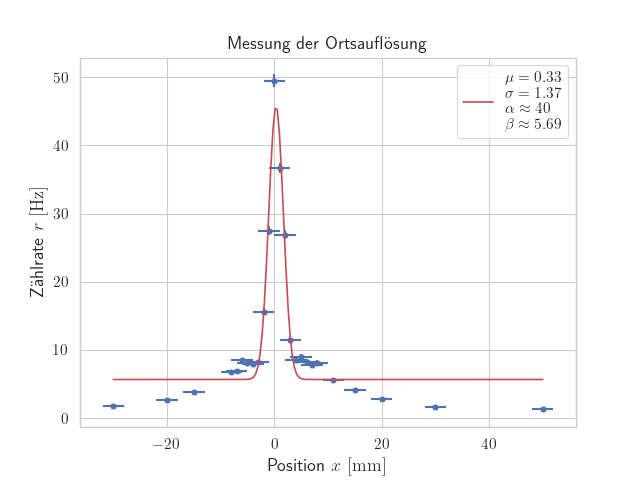
\includegraphics[width=0.9\textwidth]{../media/B3.4/Ortsaufloesung_fit.png}
	\caption{Zählraten}
	\label{abb:zaehlrate}
\end{figure}

\clearpage
\hypertarget{fazit}{%
\section{Fazit}\label{fazit}}

\clearpage
\hypertarget{literatur}{%
\section{Literatur}\label{literatur}}

\begin{enumerate}
\def\labelenumi{\arabic{enumi}.}
\tightlist
\item
  Universität zu Köln, ``B3.4: Positronen--Emissions--Tomografie'',
  Januar 2021,
  \url{https://www.ikp.uni-koeln.de/fileadmin/data/praktikum/B3.4\_PET\_de.pdf},
  Abruf am 20.03.2024
\item
  ``Chart of Nuclides'', National Nuclear Data Center,
  \url{https://www.nndc.bnl.gov/nudat3}, Abruf am 28.03.2024
\item
  ``Positronen Emissions Tomographie'', Deutsche Gesellschaft für
  Nuklearmedizin e.V., Online verfügbar unter
  \url{http://www.nuklearmedizin.de/docs/pet_bro_06.pdf}, Abruf am
  03.04.2024
\item
  W. Demtröder, ``Experimentalphysik 4: Kern-, Teilchen- und
  Astrophysik'', Springer--Spektrum--Verlag, 2017, DOI:
  \href{https://link.springer.com/book/10.1007/978-3-662-52884-6}{10.1007/978-3-662-52884-6}
\item
  Lexikon der Physik, ``Paarvernichtung'',
  \url{https://www.spektrum.de/lexikon/physik/paarvernichtung/10838},
  Abruf am 04.04.2024
\item
  Wikipedia, ``Annihilation'',
  \url{https://de.wikipedia.org/wiki/Annihilation}, Abruf am 04.04.2024
\item
  K. Bethge, Kernphysik: Eine Einführung, 3. aktualisierte und
  erweiterte Auflage, Springer--Verlag, 2008, DOI:
  \href{https://doi.org/10.1007/978-3-540-74567-9}{10.1007/978-3-540-74567-9}
\item
  Strahlenschutzkommission, ``Orientierungshilfe SSK'', 2006, ISBN 3873441306,
  \url{https://campus-nes.de/fileadmin/user_upload/Orientierungshilfe_SSK.pdf}, Abruf am 07.04.2024
\item
  Lexikon der Physik, ``Impulshöhenspektrum'',
  \url{https://www.spektrum.de/lexikon/physik/impulshoehenspektrum/7156},
  Abruf am 08.04.2024
\item
  Wikipedia,
  \url{https://de.wikipedia.org/wiki/Datei:Compton-spektrum.svg},
  Abruf am 08.04.2024
\item
  Wikipedia,
  \url{https://de.wikipedia.org/wiki/Datei:Am-Be-SourceSpectrum.jpg},
  Abruf am 08.04.2024
\item
  Wikipedia,
  \url{https://de.wikipedia.org/wiki/Datei:Photomultiplier_schema_de.png},
  Abruf am 08.04.2024
\item
  LMU München, ``Detektor'',
  \url{https://homepages.physik.uni-muenchen.de/~Otmar.Biebel/detektor/detector06.pdf},
  Abruf am 07.04.2024
\item
  Wikipedia,
  \url{https://commons.wikimedia.org/wiki/File:Constant_fraction_1.svg},
  Abruf am 06.04.2024
\item
  Wikipedia,
  \url{https://commons.wikimedia.org/wiki/File:CFD_Diagram1.jpg},
  Abruf am 06.04.2024
\item
  Wikipedia, ``Escapelinie'',
  \url{https://de.wikipedia.org/wiki/Escapelinie},
  Abruf am 08.04.2024
\end{enumerate}

\end{document}
